%DIF 1a1
%DIF LATEXDIFF DIFFERENCE FILE
%DIF DEL old.tex     Tue Jun  4 20:11:05 2019
%DIF ADD paper.tex   Tue Jun  4 18:13:46 2019
 %DIF > 
%DIF -------
\documentclass{article}
\usepackage{ijcai11}
\usepackage[dutch]{babel}
\usepackage{times}
\usepackage{gensymb}
\usepackage{graphicx}
\usepackage{float}
\usepackage{cite}
\usepackage{named}
\usepackage{url}
%DIF 11a12-13
\usepackage{csquotes} %DIF > 
\usepackage{subcaption} %DIF > 
%DIF -------
\hyphenpenalty = 10000
\exhyphenpenalty = 10000


\title{SmartLED-displays}
\author{Barbara Ameloot\\
KU Leuven\\
barbara.ameloot@student.kuleuven.be
\And 
Wouter Jochems\\
KU Leuven\\
wouter.jochems@student.kuleuven.be}
 %DIF > 
\pagenumbering{arabic} %DIF > 
%DIF PREAMBLE EXTENSION ADDED BY LATEXDIFF
%DIF UNDERLINE PREAMBLE %DIF PREAMBLE
\RequirePackage[normalem]{ulem} %DIF PREAMBLE
\RequirePackage{color}\definecolor{RED}{rgb}{1,0,0}\definecolor{BLUE}{rgb}{0,0,1} %DIF PREAMBLE
\providecommand{\DIFadd}[1]{{\protect\color{blue}\uwave{#1}}} %DIF PREAMBLE
\providecommand{\DIFdel}[1]{{\protect\color{red}\sout{#1}}}                      %DIF PREAMBLE
%DIF SAFE PREAMBLE %DIF PREAMBLE
\providecommand{\DIFaddbegin}{} %DIF PREAMBLE
\providecommand{\DIFaddend}{} %DIF PREAMBLE
\providecommand{\DIFdelbegin}{} %DIF PREAMBLE
\providecommand{\DIFdelend}{} %DIF PREAMBLE
\providecommand{\DIFmodbegin}{} %DIF PREAMBLE
\providecommand{\DIFmodend}{} %DIF PREAMBLE
%DIF FLOATSAFE PREAMBLE %DIF PREAMBLE
\providecommand{\DIFaddFL}[1]{\DIFadd{#1}} %DIF PREAMBLE
\providecommand{\DIFdelFL}[1]{\DIFdel{#1}} %DIF PREAMBLE
\providecommand{\DIFaddbeginFL}{} %DIF PREAMBLE
\providecommand{\DIFaddendFL}{} %DIF PREAMBLE
\providecommand{\DIFdelbeginFL}{} %DIF PREAMBLE
\providecommand{\DIFdelendFL}{} %DIF PREAMBLE
\newcommand{\DIFscaledelfig}{0.5}
%DIF HIGHLIGHTGRAPHICS PREAMBLE %DIF PREAMBLE
\RequirePackage{settobox} %DIF PREAMBLE
\RequirePackage{letltxmacro} %DIF PREAMBLE
\newsavebox{\DIFdelgraphicsbox} %DIF PREAMBLE
\newlength{\DIFdelgraphicswidth} %DIF PREAMBLE
\newlength{\DIFdelgraphicsheight} %DIF PREAMBLE
% store original definition of \includegraphics %DIF PREAMBLE
\LetLtxMacro{\DIFOincludegraphics}{\includegraphics} %DIF PREAMBLE
\newcommand{\DIFaddincludegraphics}[2][]{{\color{blue}\fbox{\DIFOincludegraphics[#1]{#2}}}} %DIF PREAMBLE
\newcommand{\DIFdelincludegraphics}[2][]{% %DIF PREAMBLE
\sbox{\DIFdelgraphicsbox}{\DIFOincludegraphics[#1]{#2}}% %DIF PREAMBLE
\settoboxwidth{\DIFdelgraphicswidth}{\DIFdelgraphicsbox} %DIF PREAMBLE
\settoboxtotalheight{\DIFdelgraphicsheight}{\DIFdelgraphicsbox} %DIF PREAMBLE
\scalebox{\DIFscaledelfig}{% %DIF PREAMBLE
\parbox[b]{\DIFdelgraphicswidth}{\usebox{\DIFdelgraphicsbox}\\[-\baselineskip] \rule{\DIFdelgraphicswidth}{0em}}\llap{\resizebox{\DIFdelgraphicswidth}{\DIFdelgraphicsheight}{% %DIF PREAMBLE
\setlength{\unitlength}{\DIFdelgraphicswidth}% %DIF PREAMBLE
\begin{picture}(1,1)% %DIF PREAMBLE
\thicklines\linethickness{2pt} %DIF PREAMBLE
{\color[rgb]{1,0,0}\put(0,0){\framebox(1,1){}}}% %DIF PREAMBLE
{\color[rgb]{1,0,0}\put(0,0){\line( 1,1){1}}}% %DIF PREAMBLE
{\color[rgb]{1,0,0}\put(0,1){\line(1,-1){1}}}% %DIF PREAMBLE
\end{picture}% %DIF PREAMBLE
}\hspace*{3pt}}} %DIF PREAMBLE
} %DIF PREAMBLE
\LetLtxMacro{\DIFOaddbegin}{\DIFaddbegin} %DIF PREAMBLE
\LetLtxMacro{\DIFOaddend}{\DIFaddend} %DIF PREAMBLE
\LetLtxMacro{\DIFOdelbegin}{\DIFdelbegin} %DIF PREAMBLE
\LetLtxMacro{\DIFOdelend}{\DIFdelend} %DIF PREAMBLE
\DeclareRobustCommand{\DIFaddbegin}{\DIFOaddbegin \let\includegraphics\DIFaddincludegraphics} %DIF PREAMBLE
\DeclareRobustCommand{\DIFaddend}{\DIFOaddend \let\includegraphics\DIFOincludegraphics} %DIF PREAMBLE
\DeclareRobustCommand{\DIFdelbegin}{\DIFOdelbegin \let\includegraphics\DIFdelincludegraphics} %DIF PREAMBLE
\DeclareRobustCommand{\DIFdelend}{\DIFOaddend \let\includegraphics\DIFOincludegraphics} %DIF PREAMBLE
\LetLtxMacro{\DIFOaddbeginFL}{\DIFaddbeginFL} %DIF PREAMBLE
\LetLtxMacro{\DIFOaddendFL}{\DIFaddendFL} %DIF PREAMBLE
\LetLtxMacro{\DIFOdelbeginFL}{\DIFdelbeginFL} %DIF PREAMBLE
\LetLtxMacro{\DIFOdelendFL}{\DIFdelendFL} %DIF PREAMBLE
\DeclareRobustCommand{\DIFaddbeginFL}{\DIFOaddbeginFL \let\includegraphics\DIFaddincludegraphics} %DIF PREAMBLE
\DeclareRobustCommand{\DIFaddendFL}{\DIFOaddendFL \let\includegraphics\DIFOincludegraphics} %DIF PREAMBLE
\DeclareRobustCommand{\DIFdelbeginFL}{\DIFOdelbeginFL \let\includegraphics\DIFdelincludegraphics} %DIF PREAMBLE
\DeclareRobustCommand{\DIFdelendFL}{\DIFOaddendFL \let\includegraphics\DIFOincludegraphics} %DIF PREAMBLE
%DIF LISTINGS PREAMBLE %DIF PREAMBLE
\RequirePackage{listings} %DIF PREAMBLE
\RequirePackage{color} %DIF PREAMBLE
\lstdefinelanguage{DIFcode}{ %DIF PREAMBLE
%DIF DIFCODE_UNDERLINE %DIF PREAMBLE
  moredelim=[il][\color{red}\sout]{\%DIF\ <\ }, %DIF PREAMBLE
  moredelim=[il][\color{blue}\uwave]{\%DIF\ >\ } %DIF PREAMBLE
} %DIF PREAMBLE
\lstdefinestyle{DIFverbatimstyle}{ %DIF PREAMBLE
	language=DIFcode, %DIF PREAMBLE
	basicstyle=\ttfamily, %DIF PREAMBLE
	columns=fullflexible, %DIF PREAMBLE
	keepspaces=true %DIF PREAMBLE
} %DIF PREAMBLE
\lstnewenvironment{DIFverbatim}{\lstset{style=DIFverbatimstyle}}{} %DIF PREAMBLE
\lstnewenvironment{DIFverbatim*}{\lstset{style=DIFverbatimstyle,showspaces=true}}{} %DIF PREAMBLE
%DIF END PREAMBLE EXTENSION ADDED BY LATEXDIFF

\begin{document}
\DIFdelbegin %DIFDELCMD < 

%DIFDELCMD < %%%
\DIFdelend \DIFaddbegin \fontsize{11pt}{13pt}\selectfont
\DIFaddend \maketitle

\begin{abstract}
Deze paper onderzoekt een mogelijke toepassing van SmartLEDs, LEDs aangestuurd door een microcontroller\cite{smartLED}. Specifiek bestuderen we hun mogelijkheden op het gebied van LED-displays. LED-displays kennen veel toepassingen in verschillende gebieden, zoals marketing en entertainment. De fundamentele opbouw is vaak die van een centrale aansturing die het hele display bestuurt. \DIFdelbegin \DIFdel{Dit zorgt voor enkele problemen en beperkingen }\DIFdelend \DIFaddbegin \DIFadd{Deze opbouw legt echter enkele beperkingen op en kan voor bepaalde problemen zorgen}\DIFaddend . We onderzoeken of een LED-display opgebouwd uit SmartLEDs\DIFaddbegin \DIFadd{, waarbij er geen centrale aansturing is, }\DIFaddend een meerwaarde biedt \DIFdelbegin \DIFdel{. We concluderen dat }\DIFdelend \DIFaddbegin \DIFadd{ten opzichte van de beperkingen die we bij de klassieke displays vaststellen. We evalueren de }\DIFaddend SmartLED-displays \DIFaddbegin \DIFadd{op hun flexibiliteit, hun interactiviteit en hun modulariteit. We concluderen dat, hoewel aan onze criteria wordt voldaan,  SmartLED-displays }\DIFaddend niet altijd een goede vervanging zijn voor conventionele LED-displays\DIFdelbegin \DIFdel{, maar }\DIFdelend \DIFaddbegin \DIFadd{. Ze bieden echter }\DIFaddend wel extra mogelijkheden \DIFdelbegin \DIFdel{bieden voor meer experimentelere }\DIFdelend \DIFaddbegin \DIFadd{voor meer experimentele }\DIFaddend LED-displays.
\end{abstract}

{\bf Keywords:} SmartLED, VLC, LED, LED Display, Arduino, Microcontroller,


\section{Introductie}

LED-displays worden \DIFdelbegin \DIFdel{tegenwoordig }\DIFdelend vaak gebruikt op evenementen en reclameborden. \DIFdelbegin \DIFdel{Op de markt zijn reeds flexibele alsook interactive led-displays beschikbaar. }\DIFdelend De huidige displays werken meestal met een centrale aansturing. \DIFdelbegin \DIFdel{De individuele LEDs moeten dus steeds aangesloten zijn op een soort grid om signalen te ontvangen}\DIFdelend \DIFaddbegin \DIFadd{Deze opbouw zorgt echter voor beperkingen bij het gebruik van de displays. Wij identificeren drie beperkingen waarvoor we onderzoeken of een SmartLED-display, zonder centrale aansturing, een meerwaarde kan bieden.
}

\begin{figure}
\centering
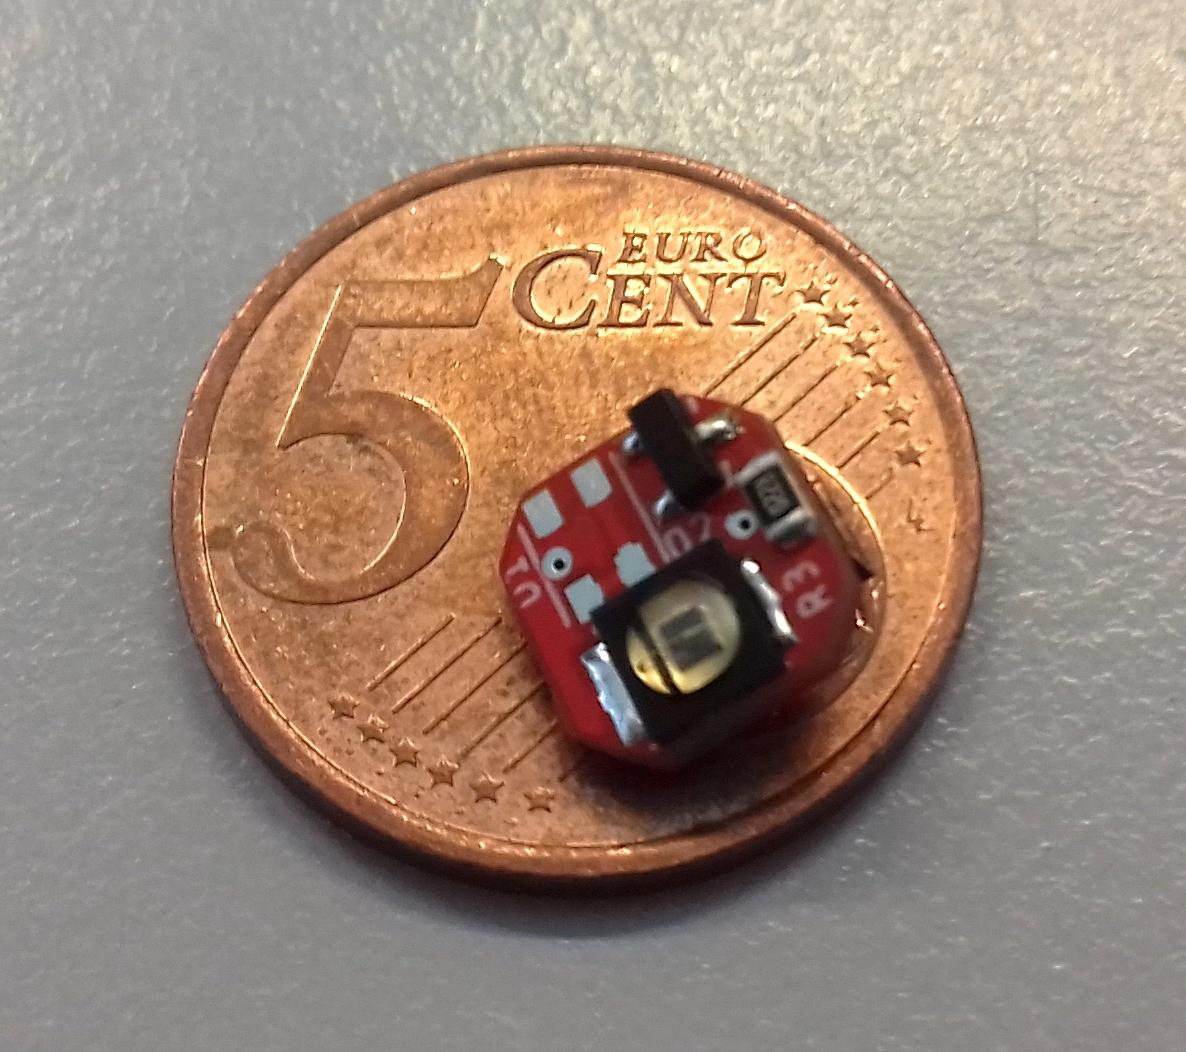
\includegraphics[width=6cm]{SmartLED.png}
\caption{\DIFaddFL{Een SmartLED}}
\end{figure}

\begin{enumerate}


\item \DIFadd{Een eerste punt is }\textbf{\DIFadd{flexibiliteit}}\DIFadd{. Er zijn reeds flexibele displays beschikbaar. Omdat elke led vanuit een centraal punt wordt aangestuurd is het nodig dat deze centrale controller kennis heeft van de positie van de LEDs}\DIFaddend . Dit zorgt ervoor dat \DIFaddbegin \DIFadd{de huidige }\DIFaddend flexibele displays beperkt zijn in hun \DIFdelbegin \DIFdel{bewegelijkheid. Bij de huidige interactive displays is het vaak zo dat het display een statisch geheel is }\DIFdelend \DIFaddbegin \DIFadd{bewegingsmogelijkheden. De individuele LEDs zijn vaak aangesloten op een raster of slinger om de relatieve positie van de LEDs ten opzichte van elkaar te behouden. Door de centrale controller weg te laten denken wij de nood aan het behouden van de relatieve posities te elimineren. Dit leidt tot meer mogelijkheden voor de dynamische flexibiliteit van een SmartLED-display}\DIFaddend .
\DIFdelbegin \DIFdel{Dit beperkt de interactie tot communicatie met een interface. De fysieke eigenschappen van het display kunnen niet aangepast worden. Bovendien zorgen problemen met de controle eenheid of met dit grid meteen voor significante storingen in het display \mbox{%DIFAUXCMD
\cite{brokenDisplay} }\hspace{0pt}%DIFAUXCMD
waardoor vaak het hele display zo goed als onbruikbaar wordt.
}%DIFDELCMD < \begin{figure}
%DIFDELCMD < %%%
\DIFdelendFL \DIFaddbeginFL 

\item \DIFaddFL{Een tweede punt is }\textbf{\DIFaddFL{interactiviteit}}\DIFaddFL{. Ook hier zijn er reeds interactieve displays op de markt. Deze zijn echter vaak rigide. Door elke SmartLED van een eigen micro-controller te voorzien zorgen we ervoor dat deze zelf signalen van buitenaf kan verwerken. De individuele LEDs zijn bijgevolg onafhankelijk van andere besturingselementen toch in staat om in interactie te treden met de buitenwereld. Voor deze interactie maken we gebruikt van een “lichtpen”, dit is een SmartLED die een gebruiker op het display kan richten om zo signalen over te brengen aan de hand van infrarood licht.
}

\item \DIFaddFL{Als derde en laatste punt bekijken we }\textbf{\DIFaddFL{modulariteit}}\DIFaddFL{. Zoals eerder vermeld is de flexibiliteit van de huidige displays beperkt. Doordat de LEDs vanuit \'e\'en centraal punt worden aangestuurd zullen problemen bij de centrale controller een impact hebben op het hele display. Ook is het vaak moeilijk om een individuele LED of groepen van LEDs te vervangen wanneer deze niet meer werken. Door elke SmartLED als individuele entiteit te laten functioneren kunnen problemen zich niet voortplanten over het display. Omdat de SmartLEDs enkel afhankelijk zijn van zichzelf is het ook makkelijk om een enkele led te vervangen.
}\end{enumerate}

\begin{figure}[H]
\DIFaddendFL \centering
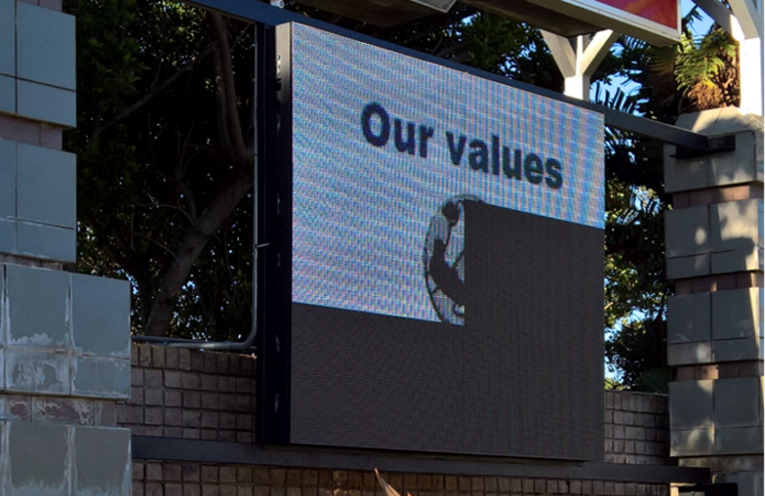
\includegraphics[width=8cm]{broken.png}
\DIFdelbeginFL %DIFDELCMD < \caption{%
{%DIFAUXCMD
\DIFdelFL{Een LED-display met verbindingsproblemen}}
%DIFAUXCMD
\DIFdelendFL \DIFaddbeginFL \caption[Een LED-display met verbindingsproblemen]{\DIFaddFL{Een LED-display met verbindingsproblemen \mbox{%DIFAUXCMD
\cite{brokenDisplay}}\hspace{0pt}%DIFAUXCMD
}}
\DIFaddendFL \end{figure}

\DIFdelbegin \DIFdel{Smart LEDs kunnen een oplossing bieden voor deze problemen. Elke LED beschikt namelijk over zijn eigen microcontroller. Dit verwijdert de nood aan verbinding met een grid aangezien de besturing bij de LED zelf gebeurd. Hierdoor krijgen de LEDs meer bewegingsvrijheid en wordt het makkelijker om delen van het display te vervangen . Daarbij beperken storingen ten gevolge van controllerproblemen zich tot slechts 1 LED waardoor reparaties aan het displaybeperkter zijn. Verder kunnen SmartLEDs samen werken door met elkaar te communiceren. Dit gebeurt via VLC (}\textit{\DIFdel{Visual Ligth Communication}}%DIFAUXCMD
\DIFdel{) waarbij visueel licht gebruikt wordt om informatie door te zenden\mbox{%DIFAUXCMD
\cite{VLC}}\hspace{0pt}%DIFAUXCMD
.
Hiervoor gebruiken ze hun ingebouwde LED die zowel als zender als als ontvanger kan dienen. 
}%DIFDELCMD < 

%DIFDELCMD < %%%
\DIFdelend \section{Verwant werk}
Dit project is een rechtstreeks vervolg op het project van vorig jaar waarin de SmartLEDs ontwikkeld werden. \DIFdelbegin %DIFDELCMD < 

%DIFDELCMD < %%%
\DIFdelend \DIFaddbegin \DIFadd{\mbox{%DIFAUXCMD
\cite{smartLED}
}\hspace{0pt}%DIFAUXCMD
}\DIFaddend Daarnaast is er al veel onderzoek gebeurd rond LEDs en hun mogelijk tot signaaloverdracht. Zo werd er al door ETH Zurich en Disney research onderzoek gedaan naar de mogelijkheden van VLC\DIFaddbegin \DIFadd{, visual light communication, }\DIFaddend networks waarbij verschillende microcontrollers met elkaar communiceerden via LEDs \cite{VLCNetworks}.  \DIFaddbegin \DIFadd{Verder is er nog project firefly\mbox{%DIFAUXCMD
\cite{firefly} }\hspace{0pt}%DIFAUXCMD
waarbij reeds een werkend display werd opgebouwd van individueel aangestuurde LEDs maar deze waren nog steeds verbonden via een kabel.
}\DIFaddend 



\section{Evaluatie}

Het doel van ons onderzoek is nagaan of een display opgebouwd uit SmartLEDs een meerwaarde biedt ten opzichte van gewone displays. \DIFdelbegin \DIFdel{We gaan na welke problemen opduiken en onderzoeken hier oplossingen voor.
}%DIFDELCMD < 

%DIFDELCMD < %%%
\DIFdel{Onze belangrijkste criteria zijn de flexibiliteit van het display en de mogelijkheid tot interactie met het display. Met flexibiliteit }\DIFdelend \DIFaddbegin \DIFadd{Hiervoor bekijken we de drie beperkingen die we vaststellen bij de klassieke displays: flexibiliteit, interactiviteit en modulariteit. Daarnaast onderzoeken we welke bijkomende beperkingen een SmartLED-display heeft.
}

\DIFadd{Met }\textbf{\DIFadd{flexibiliteit}} \DIFaddend bedoelen we dat het mogelijk moet zijn om de SmartLEDs te verplaatsen zonder dat hiervoor code moet worden aangepast. Dit betekent dat de communicatie met en door de SmartLEDs onafhankelijk moeten werken van hun positie in het display. 

Voor de \DIFdelbegin \DIFdel{interactie }\DIFdelend \DIFaddbegin \textbf{\DIFadd{interactie}} \DIFaddend willen we dat deze op een betrouwbare en interactieve manier gebeurt. Hiervoor maken we gebruik van een "lichtpen". Dit is een SmartLED voorzien van enkele knoppen om zo input door te sturen naar het display. Aan de hand van een floodlight, een lichtpen voorzien van meerdere, krachtigere LEDs, kunnen grotere groepen SmartLEDs aangestuurd worden. \DIFaddbegin \DIFadd{Het moet dus mogelijk zijn om aan de hand van een SmartLED een signaal te geven aan een andere SmartLED.
}\DIFaddend 

\DIFaddbegin \DIFadd{Voor }\textbf{\DIFadd{modulariteit}} \DIFadd{is het belangrijk dat er SmartLEDs kunnen worden toegevoegd en weggelaten zonder dat dit een invloed heeft op de rest van het display. Dit hangt nauw samen met de flexibiliteit. Waar we bij flexibiliteit vooral kijken naar de verplaatsbaarheid van LEDs, leggen we hier de focus op het toevoegen en weglaten van SmartLEDs. Hier is het vooral belangrijk dat het niet uitmaakt welke LEDs er deel uitmaken van het display. 
}



\DIFaddend \section{\DIFdelbegin \DIFdel{Implementatie}%DIFDELCMD < \MBLOCKRIGHTBRACE
%DIFDELCMD < %%%
\DIFdel{Om }\DIFdelend \DIFaddbegin \DIFadd{Opstelling}}
\DIFadd{De uiteindelijke implementatie zou gebruik maken van SmartLEDs. Om praktische redenen waren wij niet in staat deze te gebruiken tijdens ons onderzoek. 
Om }\DIFaddend onze hypothese te testen \DIFdelbegin \DIFdel{maakten }\DIFdelend \DIFaddbegin \DIFadd{maken }\DIFaddend we gebruik van LEDs verbonden met Zigduino r2 microcontrollers. \DIFdelbegin \DIFdel{We maakten gebruik van infrarood LEDs voor de communicatie om extra lichtflikkeringen in het display te voorkomen en om interferentie van de omgeving zo veel mogelijk te vermijden. }\DIFdelend \DIFaddbegin \DIFadd{De Zigduino’s bevatten een infrarood led en een RGB led. We kiezen ervoor om een infrarood led toe te voegen omdat dit de communicatie een stuk minder complex maakt. Indien we gebruik zouden maken van zichtbaar licht, zoals bij VLC, is het nodig om rekening te houden met het omgevingslicht. Dit veranderd voortdurend en deze verandering moet in rekening gebracht worden om onderscheidt te maken van een doelbewust signaal en het aanwezige omgevingslicht. De veranderingen in het aanwezige infrarood licht zijn veel minder uitgesproken. Dit laat ons toe om de threshold, de waarde vanaf wanneer we een signaal registreren, redelijk constant te houden. Om deze reden stappen we af van de pure VLC en kiezen we ervoor een extra infrarood LED toe te voegen.
}\DIFaddend 

\DIFdelbegin \section{\DIFdel{Oplossing}}
%DIFAUXCMD
\addtocounter{section}{-1}%DIFAUXCMD
\DIFdelend \DIFaddbegin \begin{figure}[H]
\centering
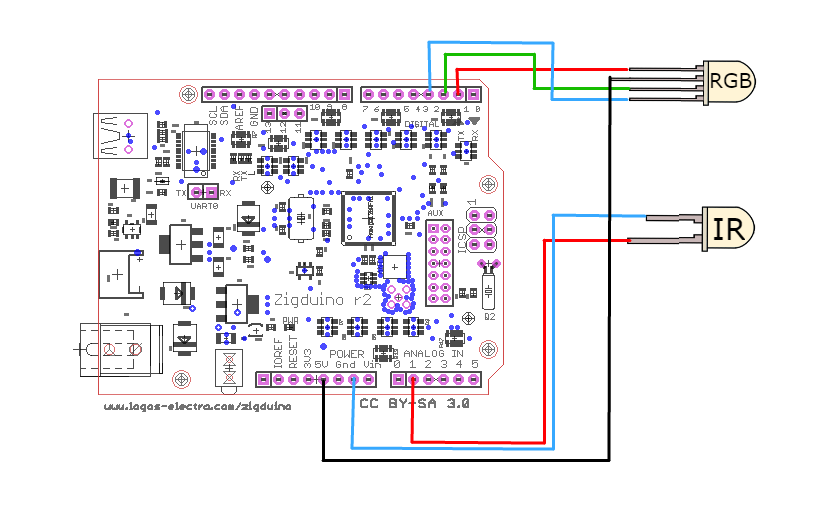
\includegraphics[width=9cm]{Opstelling.png}
\caption{\DIFaddFL{De opstelling voor de display SmartLEDs}}
\label{fig:opstelling}
\end{figure}
\DIFaddend 


\DIFdelbegin \subsection{\DIFdel{Onderlinge communicatie}}
%DIFAUXCMD
\addtocounter{subsection}{-1}%DIFAUXCMD
\DIFdel{Om een vlak display te bekomen, moeten de LEDs uiteraard zijdelings staan. Dit zorgde helaas voor problemen, aangezien elke LED een specifieke invalshoek heeft. Wij hadden echter geen LEDs met een hoek van 180}%DIFDELCMD < \degree %%%
\DIFdel{ter beschikking.
 Als oplossing probeerden we een diffuser te gebruiken maar hierdoor verzwakte het licht van onze LEDs waardoor er geen signaal kon worden verzonden. Mogelijk zou dit geen probleem zijn bij sterkere LEDs maar deze zouden problemen kunnen geven omdat ze teveel energie vragen. 
}\DIFdelend \DIFaddbegin \section{\DIFadd{Methode}}
\DIFaddend 

\DIFdelbegin \DIFdel{Met twee naar elkaar gerichte LEDs lukt het ons wel om een bit-string door te zenden. Deze opstelling bestaat uit een eerste LED die een bit-string uitzendt, een tweede die deze ontvangt }\DIFdelend \DIFaddbegin \DIFadd{Voor het schrijven van de code}\footnote{\DIFadd{Alle code is beschikbaar op }\\ \DIFadd{https://github.com/WoodyJo/SmartLED-displays}} \DIFadd{gebruiken we de standaard Arduino IDE, aangepast om te werken met Zigduino's. De experimenten zijn gedaan met Zigduino r2 microcontrollers. Bij de applicaties beschreven in sectie \ref{interactie} hebben we een pingpongbal over de LEDs geplaatst om het zichtbaar licht duidelijker te maken. Dit gaf geen hinder voor de communicatie.
}

\DIFadd{We zoeken eerst een methode om signalen door te geven over verschillende SmartLEDs. Hiervoor baseren we ons op het werk van \mbox{%DIFAUXCMD
\cite{smartLED}}\hspace{0pt}%DIFAUXCMD
. Daarna bekijken we de mogelijkheden voor communicatie voor de voor ons 2 relevante aspecten: zijwaartse communicatie voor de LEDs in het display; en face-to-face voor interactie met een gebruiker.
 }

\DIFadd{Ook bekijken we 2 manieren voor interactie met het display. De eerste manier werkt op een heel simpele manier en registreert slechts 1 soort input; er wordt een lichtpen op het display gericht. De tweede manier maakt gebruik van de signaaloverdracht zoals die beschreven wordt; er wordt een bitstring overgedragen. 
}

\section{\DIFadd{Signaaloverdracht}}\label{signaaloverdracht}

\DIFadd{Voor de communicatie tussen SmartLEDs zijn we vertrokken vanuit VLC, visual light communication. Zoals \mbox{%DIFAUXCMD
\cite{VLCNetworks} }\hspace{0pt}%DIFAUXCMD
aantoont is het mogelijk om LEDs te gebruiken om zowel licht uit te zenden als te ontvangen. Dit kan gebruikt worden voor communicatie tussen LEDs onderling zonder dat dit merkbaar is voor een gebruiker; de LED lijkt altijd aan, zo blijkt uit de paper. De communicatie verloopt grotendeels zoals beschreven in \mbox{%DIFAUXCMD
\cite{smartLED}}\hspace{0pt}%DIFAUXCMD
. Met als uitzondering de schakeling van de LED. 
}

\DIFadd{De signaaloverdracht gebeurt aan de hand van infrarood licht. Een zender SmartLED zend een bitstring uit via on-off keying. Hierbij wordt de binaire “1” voorgesteld door de LED aan te zetten en de “0” door de LED uit te zetten. Afhankelijk van de ontvangen bitstring zal de ontvanger de bijhorende reactie ondernemen. (zie figuur \ref{fig:onfoff}).
}

\begin{figure}[H]
\centering
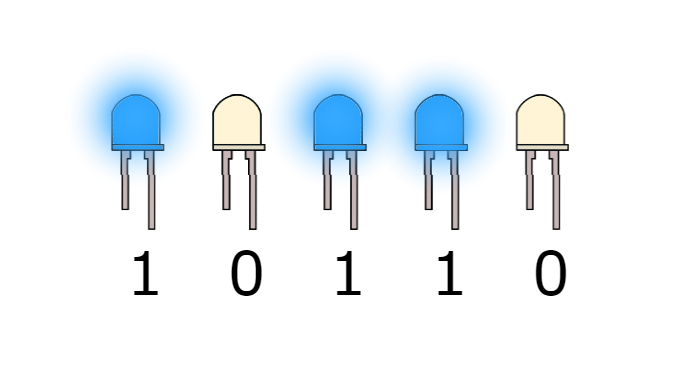
\includegraphics[width=8cm]{OnOff.png}
\caption{\DIFaddFL{on-off keying}}
\label{fig:onfoff}
\end{figure}

\subsection{\DIFadd{Reverse Bias}}
\DIFadd{We hebben gemerkt dat het verschil tussen de gemeten waarde wanneer we wel of niet op de LED schijnen veel groter is wanneer we de infrarood LED in }\textbf{\DIFadd{reverse bias}} \DIFadd{schakelden, in tegenstelling tot de forward bias zoals in \mbox{%DIFAUXCMD
\cite{smartLED} }\hspace{0pt}%DIFAUXCMD
gebruikt wordt. Dit vermoeden wordt bevestigd door de resultaten in tabel 1. Deze geeft telkens de waarden weer die door de Zigduino over de LED worden gemeten. Zoals beschreven in de Arduino Referentie \mbox{%DIFAUXCMD
\cite{Arduino} }\hspace{0pt}%DIFAUXCMD
bevat het bord een analog to digital converter. Deze mapt het input voltage op integer waarden tussen 0 }\DIFaddend en \DIFdelbegin \DIFdel{doorgeeft aan een microcontroller en vervolgens een derde die de ontvangen bit-string weer uitzendt in een andere richting. In minder conventionele LED-displays (met een vorm die het toelaat de LEDs naar een elkaar te richten of met bewegende onderdelen)is onderlinge communicatie dus wel mogelijk}\DIFdelend \DIFaddbegin \DIFadd{1023. Bij de Zigduinos gebeurt dit op dezelfde manier. De tabel geeft een gemiddelde van 30 metingen van deze integer waarden zoals gemeten met de lichtbron op verschillende afstanden, alsook zonder de lichtbron}\DIFaddend . 

\DIFaddbegin \DIFadd{Om het verschil tussen de forward bias en reverse bias te bevestigen bekijken we de waarden voor een afstand van 8 cm. Dit lijkt ons een representatieve afstand voor de communicatie met de lichtpen. We bekijken het absolute verschil tussen de waardes met en de waardes zonder lichtbron. 
Voor de forward bias zien we een absoluut verschil van 27. Dit bedraagt slechts 6,96\% van de standaardwaarde zonder licht. 
Voor de reverse bias zien we een absoluut verschil van 712, ofwel 98,6\% van de standaardwaarde zonder licht. 
Door het grote verschil in waarde is het makkelijker om te registreren wanneer er effectief een signaal naar de LED wordt gestuurd in plaats van eventuele ruis. We plaatsen de infrarood LED dus in reverse bias.
}


\begin{table}
	\centering
    \begin{tabular}{ | p{1.5cm} | p{1.5 cm} | p{1.5 cm} | }
    \hline
    & & \\
    \DIFaddFL{Afstand tot lichtbron (in cm) }& \DIFaddFL{Reverse Bias gemeten waarde }& \DIFaddFL{Forward Bias gemeten waarde  }\\ \hline
    & &  \\
    \DIFaddFL{4 }& \DIFaddFL{0 }& \DIFaddFL{425  }\\ 
    \DIFaddFL{6 }& \DIFaddFL{3 }& \DIFaddFL{418   }\\ 
    \DIFaddFL{8 }& \DIFaddFL{10 }& \DIFaddFL{416   }\\ 
    \DIFaddFL{10 }& \DIFaddFL{24 }& \DIFaddFL{413   }\\ 
    \DIFaddFL{15 }& \DIFaddFL{330 }& \DIFaddFL{405   }\\ 
    \DIFaddFL{20 }& \DIFaddFL{380 }& \DIFaddFL{397  }\\ 
    \DIFaddFL{30 }& \DIFaddFL{515 }& \DIFaddFL{388  }\\ \hline
    & & \\ 
    \DIFaddFL{Geen extra lichtbron }& \DIFaddFL{722 }& \DIFaddFL{388   }\\ 

    \hline
    \end{tabular}
  \caption{\DIFaddFL{Gemeten waarden over LED}} 
\end{table}

\subsection{\DIFadd{Synchronisatie}}\label{synch}

 \DIFadd{Voor de }\textbf{\DIFadd{synchronisatie}} \DIFadd{maken we gebruik van oversampling, zoals beschreven in de paper. Dit houdt in dat we voor elke bit meerdere lezingen uitvoeren, namelijk 3. Door de metingen met elkaar te vergelijken kunnen onverwachte veranderingen worden opgespoord. Hieruit kan worden afgeleid of de lezer voor of achterloopt op de zender. Om ervoor te zorgen dat de juiste bitstring gelezen wordt, zal de lezer de fout corrigeren door de laatste meting van de vorige bit over te brengen naar de volgende. Voor de volgende bit worden dan maar 2 bijkomende metingen gedaan.
 }

\DIFadd{Om het begin van de bitstring aan te geven gebruiken we een preamble. Deze bestaat simpelweg uit drie een’en gevolgd door een nul. De ontvanger controleert of hij deze preamble ontvangt en indien dit het geval is, begint hij de bitstring te registreren.
}

\subsection{\DIFadd{Threshold}}

\DIFadd{Om ervoor te zorgen dat de SmartLEDs een verschil zien tussen omgevingslicht en een signaal moeten we een threshold, een waarde vanaf wanneer we een meeting als input beschouwen, instellen. Omdat we gebruik maken van infraroodlicht blijft de waarde van de threshold redelijk constant. We merken echter wel verschillen in de gemeten basiswaarde afhankelijk van het gebruikte Zigduino-bord en eventuele storingsbronnen. Hierdoor is het nodig om op regelmatige tijdstippen de waarde van de threshold bij te sturen. 
Wanneer we de gemeten waarde zonder lichtinput plotten krijgen we een duidelijk sinusoïdale verloop zoals te zien op figuur \ref{fig:ruis}. Dit valt te verklaren door de RC-kringen in de gebruikte zigduino’s die als oscillator werken. \mbox{%DIFAUXCMD
\cite{oscillator}  
}\hspace{0pt}%DIFAUXCMD
}

\begin{figure}[H]
\centering
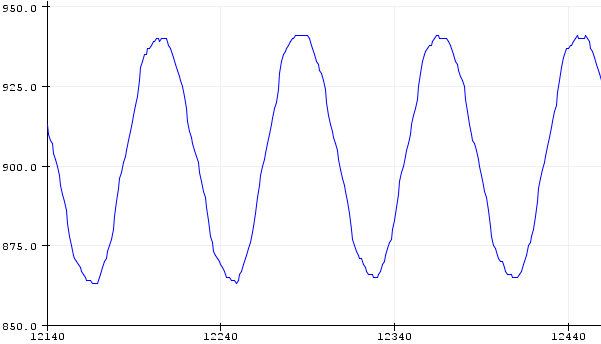
\includegraphics[width=8cm]{ruis.png}
\caption{\DIFaddFL{De gedetecteerde ruis, gemeten spanning in functie van de tijd}}
\label{fig:ruis}
\end{figure}

\DIFadd{Om de gemeten waarde van het omgevingslicht nauwkeuriger te maken besloten we om deze gelijk te stellen aan het gemiddelde van tien metingen met telkens 50ms (ongeveer de helft van een periode) tussen om het sinuso\"idale verloop op te vangen. Hierbij tellen we een waarde op, die groter is dan de amplitude van de sinus golf, en bekomen zo onze threshold. 
Voor ons onderzoek volstaat het om de threshold te bepalen wanneer de SmartLED wordt geactiveerd of een nieuw programma wordt uitgevoerd.
}

\section{\DIFadd{Communicatie}}\label{communicatie}
\subsection{\DIFadd{Face-to-face Communicatie}}
\DIFadd{Wanneer we twee SmartLEDs naar elkaar richten (zoals in figuur \ref{fig:plaatsingFace}), kunnen we aan de hand van de eerder beschreven technieken een bitstring verzenden. Dit kunnen we gebruiken om via een lichtpen, een SmartLED die voorzien is van besturingsknoppen, een signaal door te sturen naar de andere SmartLEDs. 
}

\begin{figure}
\centering
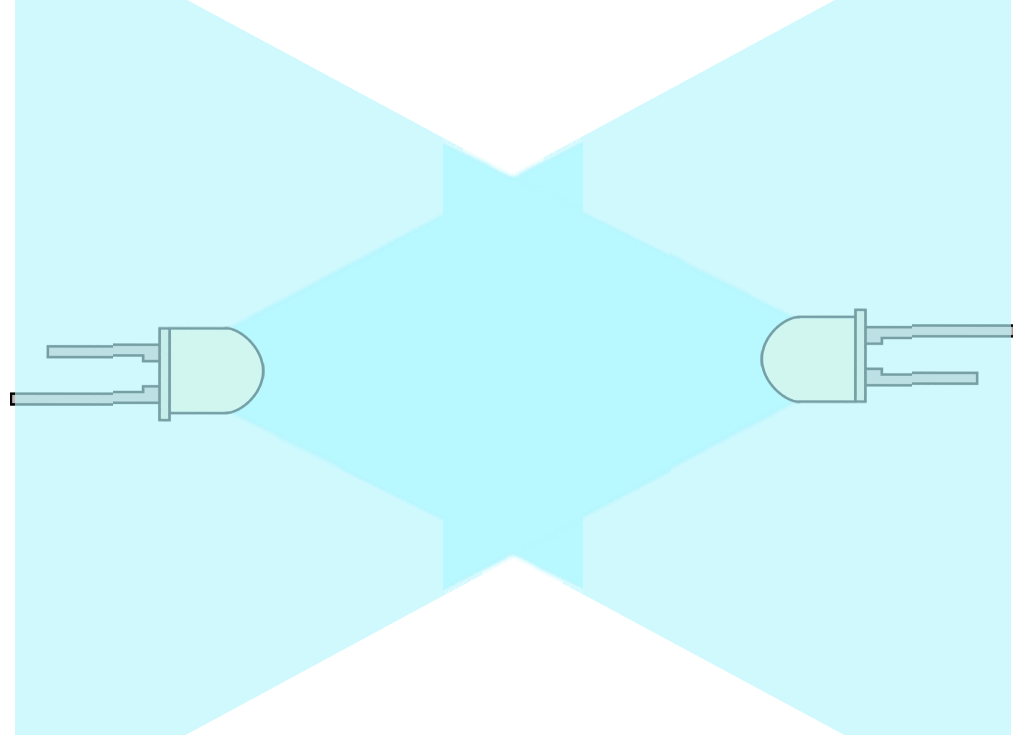
\includegraphics[width=7cm]{LedTegenoverElkaar.png}
\caption{\DIFaddFL{Stralingshoek bij Face-to-Face gepositioneerde LEDs}}
\label{fig:plaatsingFace}
\end{figure}

\subsection{\DIFadd{Zijwaartse Communicatie}}
\DIFadd{Om de LEDs als \'e\'en display te laten werken, zoeken we een manier om een signaal door te geven tussen de LEDs. Hiervoor wilden we aanvankelijk gebruik maken van de aanwezige infrarood LED. We zijn er echter niet in geslaagd om een zijdelings signaal door te geven indien de LEDs beiden naar boven wijzen. Dit is te verklaren door de beperkte stralingshoek van de LED, zoals ge\"illustreerd in figuur \ref{fig:plaatsing}.
}

\begin{figure}[H]
\centering
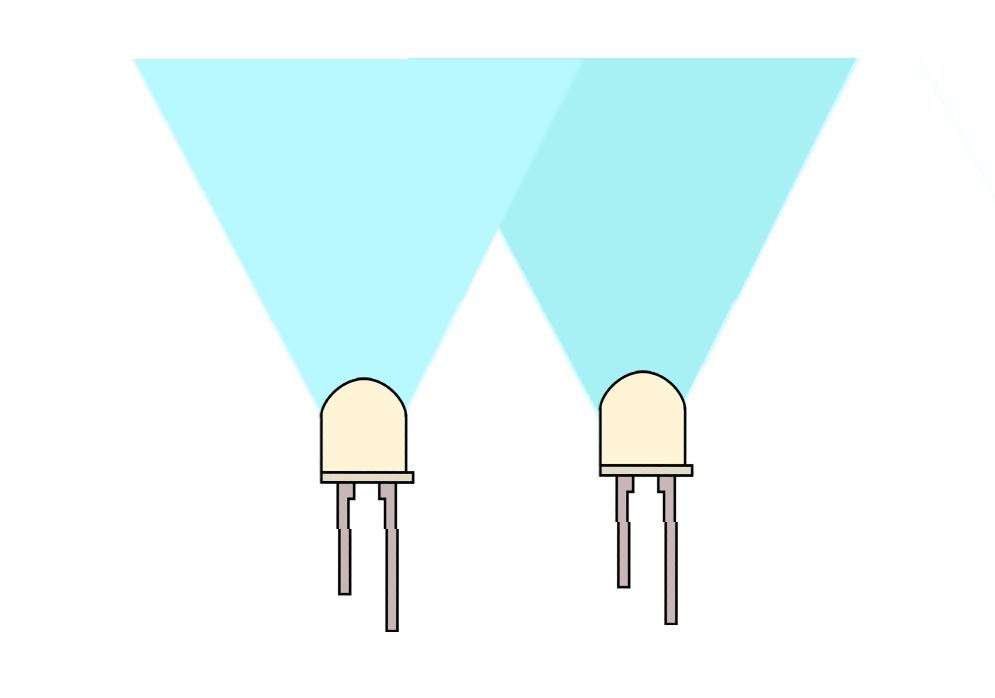
\includegraphics[width=8cm]{LedNaastElkaar.png}
\caption{\DIFaddFL{Stralingshoek bij zijdelings gepositioneerde LEDs}}
\label{fig:plaatsing}
\end{figure}

\DIFadd{Een mogelijke oplossing hiervoor zou het gebruiken van een diffuser kunnen zijn om zo een grotere stralingshoek te bekomen. Wij hebben dit in onze opstelling getest aan de hand van een pingpong bal. Dit bleek in ons geval echter niet voldoende om de zijwaartse communicatie te doen slagen. Door een krachtigere LED te gebruiken, d.w.z. een die meer lumen produceert, zou dit mogelijk toch een oplossing kunnen zijn. Dit hebben wij niet verder onderzocht. 
}

\DIFadd{Een andere mogelijkheid zou zijn om dit op te lossen door extra infrarood LEDs te monteren die naar de buitenkant gericht zijn, in plaats van naar boven. Wij hebben er echter voor gekozen dit niet te doen omdat we de SmartLEDs zo eenvoudig mogelijk wilden houden. 
}

\DIFadd{Deze keuze resulteert echter wel in een beperking voor eventuele toepassingen van het display:
}\medskip
\begin{displayquote}

 \textit{\DIFadd{Er is geen zijwaartse communicatie tussen de individuele SmartLEDs.}}
\end{displayquote}
\medskip

\DIFadd{Om de LEDs toch als 1 geheel te laten werken stellen wij een systeem voor dat gebruik maakt van een floodlight. Dit is een SmartLED die is uitgerust van meerdere infrarood LEDs zodat deze in staat is om over een groter oppervlak te schijnen. Dit maakt het mogelijk om de display-SmartLEDs te synchroniseren en gelijktijdig een bepaald programma te laten starten. Omdat de LEDs zonder onderlinge communicatie waarschijnlijk niet perfect synchroon zullen blijven, is het nodig hier rekening mee te houden bij de keuze van de toepassing. 
}




\DIFaddend \subsection{Meerdere LEDs}
Bij aanvang van ons project hoopten we voor het display en het verzenden van informatie dezelfde LED te gebruiken. Dit is niet alleen \DIFdelbegin \DIFdel{compacter dan met meerdere LEDs }\DIFdelend \DIFaddbegin \DIFadd{compact, }\DIFaddend maar het zorgt er ook voor dat we de SmartLED niet moeten uitbreiden met extra hardware. \DIFdelbegin \DIFdel{Helaas bracht dit extra moeilijkheden met zich mee, zoals informatie die verzonden moest worden over een LED die volgens het display geen licht mag uitzenden. Ook maakte dit onze code veel complexer en  
}\DIFdelend \DIFaddbegin \DIFadd{We hebben echter besloten om een tweede LED, namelijk een infrarood LED, te gebruiken omdat dit de communicatie een stuk eenvoudiger laat verlopen  zoals beschreven bij de threshold. 
}\DIFaddend 

Om \DIFdelbegin \DIFdel{deze redenen kozen we om met een tweede LED te werken. Ook besloten we om de communicatie via een infrarood LED te laten verlopen, zo vermijden we dat de communicatie-LEDs signalen zouden opvangen van de display-LEDs. Bovendien creëert dit meer mogelijkheden voor het display aangezien het volledige RGB spectrum kan gebruikt worden om afbeeldingen weer te geven. }\DIFdelend \DIFaddbegin \DIFadd{visuele redenen hebben we ervoor gekozen om als display-LED een RGB LED te gebruiken. Dit laat ons toe om via \'e\'en enkele LED meer te vari\"eren in de informatie die we kunnen overbrengen naar de gebruiker. Zo zijn kleuren in staat om emotionele reacties op te wekken \mbox{%DIFAUXCMD
\cite{color}}\hspace{0pt}%DIFAUXCMD
. Omdat we voor een SmartLED display vooral een toepassing zien in marketing en entertainment vinden we de hogere kost van een RGB LED verantwoord. Kleuren spelen een belangrijk instrument in marketing \mbox{%DIFAUXCMD
\cite{marketing}}\hspace{0pt}%DIFAUXCMD
.
}\DIFaddend 

\DIFdelbegin \subsection{\DIFdel{Externe lichtbron}}
%DIFAUXCMD
\addtocounter{subsection}{-1}%DIFAUXCMD
\DIFdel{Omdat een tweede LED ook een externe lichtbron is, valt uit het voorgaande al te besluiten dat een goed gericht licht in staat is om te interageren met een SmartLED-display. }%DIFDELCMD < 

%DIFDELCMD < %%%
\DIFdel{Wij onderzochten twee manieren waarop }\DIFdelend \DIFaddbegin \section{\DIFadd{Interactie}}\label{interactie}
\DIFadd{Zoals eerder vermeld maken we voor de }\DIFaddend interactie met het \DIFdelbegin \DIFdel{LED-display mogelijk was. Dit aan de hand }\DIFdelend \DIFaddbegin \DIFadd{display gebruik }\DIFaddend van een lichtpen\DIFdelbegin \DIFdel{(een LED met een microcontroller achter) die op een bepaalde manier geprogrammeerd was. }%DIFDELCMD < 

%DIFDELCMD < %%%
\DIFdelend \DIFaddbegin \DIFadd{. Deze interactie kan op twee manieren verlopen. }\DIFaddend De eerste manier \DIFdelbegin \DIFdel{bestond uit een reactie van het display wanneer een signaalverzonden werd, versus wanneer er geen verzonden werd. We programmeerden hiervoor een soort }\DIFdelend \DIFaddbegin \DIFadd{maakt gebruik van een heel simpele aanpak. Hierbij kijkt het display enkel naar de aan- of afwezigheid van een signaal. Dit noemen wij de }\DIFaddend "\DIFaddbegin \DIFadd{Na\"ive Methode". Voor de tweede manier maken we gebruik van de communicatiemethode zoals eerder beschreven (in sectie \ref{communicatie}). Deze methode noemen wij de "Bitstring Methode".
}

\subsection{\DIFadd{Na\"ive Methode}}

\DIFadd{Voor de na\"ive methode is er geen nood aan de synchronisatie zoals beschreven in \ref{synch}. De display-SmartLEDs registreren elke waarde die de threshold overschrijdt al input. Deze vorm van communicatie stelt ons al in staat enkele simpele toepassingen te implementeren.
}

\subsubsection{\DIFadd{Verfborstel}}
\DIFadd{Een eerste toepassing is een verfborstel applicatie. Deze vorm van interactie is volledig afhankelijk van de input van de gebruiker; de SmartLEDs nemen zelf geen initiatief.
}

\DIFadd{Bij de start van het programma staan de display-LEDs op wit. Wanneer de lichtpen voorbij komt veranderen ze van kleur, naar blauw. Deze kleur houden ze enkele seconden aan waarna ze weer naar wit overschakelen. Wanneer we meerdere display-LEDs naast elkaar zetten zijn we in staat een groter canvas te maken. Door de aard van de toepassing is het niet nodig om synchronisatie te voorzien tussen de individuele SmartLEDs. Voor de gebruiker werkt het canvas als \'e\'en geheel.
}


\subsubsection{\DIFadd{Whack-a-Mole}}
\DIFadd{Voor een tweede toepassing met de na\"ive methode wilden we de interactiemogelijkheden testen met behulp van een interactief spel. Hierbij nemen de SmartLEDs wel initiatief en wordt hun volgende actie bepaald afhankelijk van de actie van de gebruiker. 
}

\DIFadd{We kozen hier voor een variant op "}\DIFaddend \textit{\DIFdelbegin \DIFdel{Whack-a-mole}\DIFdelend \DIFaddbegin \DIFadd{Whack-a-Mole}\DIFaddend }" \DIFdelbegin \DIFdel{spel waarbij de speler een bepaalde tijd heeft om te reageren op een licht verandering door de lichtpen hierover te laten schijnen. Zowel bij succes als bij mislukking geeft het display feedback door weer van licht te veranderen (zie figuur \ref{fig:mole}).
}%DIFDELCMD < \begin{figure}
%DIFDELCMD < %%%
\DIFdelendFL \DIFaddbeginFL \DIFaddFL{(zie figuur \ref{fig:mole}). Hier staan de display-LEDs bij de start van het programma op groen. Na een willekeurig bepaalde tijd veranderen ze van kleur, naar rood, om aan te geven dat de gebruiker actie moet ondernemen. Indien de gebruiker de lichtpen op de display-LED richt zal deze de input registreren en even overgaan naar blauw om aan te geven dat de rode LED succesvol is “uitgeschakeld”. Indien er binnen de twee seconden geen input wordt geregistreerd betekend dit dat de rode LED niet is uitgeschakeld en zal de display-LED dit aangeven door oranje te knipperen.  
Ook hier is er geen nood aan synchronisatie, de willekeurige aard van het spel laat toe om de individuele Smart-LEDs als een gesimuleerd geheel te laten werken voor de gebruiker.
}


\begin{figure}[H]
\DIFaddendFL \centering
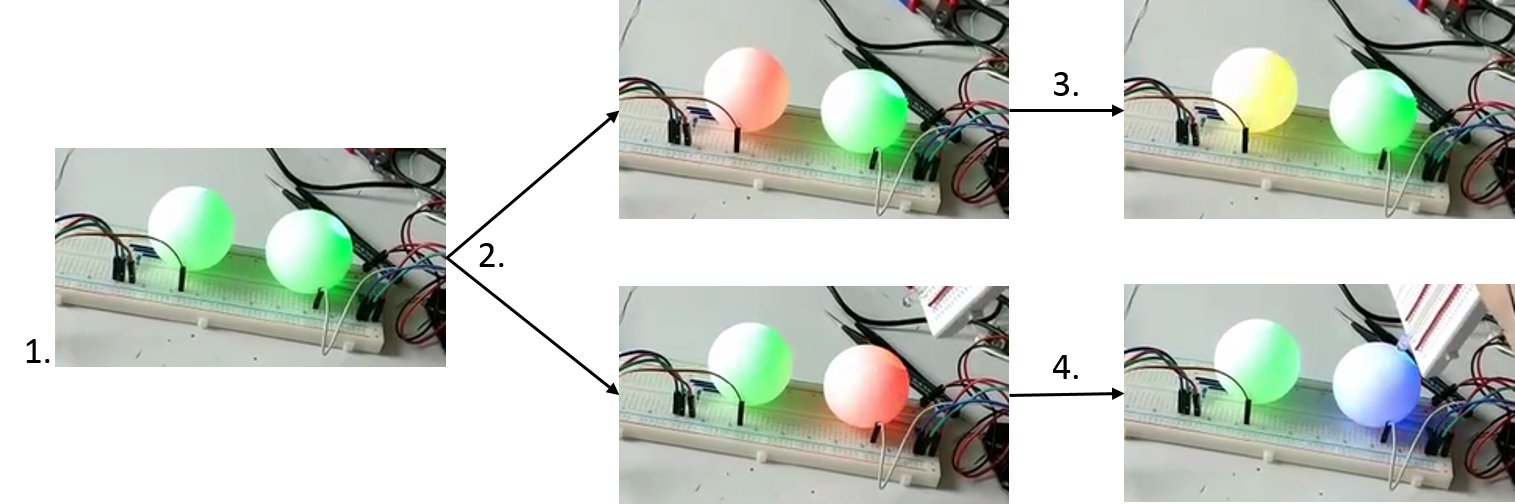
\includegraphics[width=8cm]{moleSequence.png}
\caption{\DIFaddbeginFL \DIFaddFL{Whack-a-Mole; }\DIFaddendFL 1:inactief, 2:vraagt om respons, 3:geen respons, \mbox{4: wel respons}}
\label{fig:mole}
\end{figure}

\DIFdelbegin \DIFdel{Bij de }\DIFdelend \DIFaddbegin \subsection{\DIFadd{Bitstring Methode}}


\DIFadd{Bij de bitstring methode hebben de lichtpen voorzien van drie knoppen. Deze knoppen hebben elk hun eigen unieke bistring. Dit laat ons toe om meer interactiemogelijkheden te gebruiken bij de implementatie. 
}

\subsubsection{\DIFadd{Verfborstel 2}}
\DIFadd{We hebben de verfborstel applicatie uitgebreid met deze nieuwe mogelijkheden. Elke knop komt nu overeen met een kleur: rood, groen en blauw. Wanneer de gebruiker een knop indrukt zal de display-LED de overeenkomstige kleur aannemen. Na enkele seconden wordt de LED terug wit. Ook is het mogelijk om aan een combinatie van knoppen een bitstring toe te kennen. Zo kunnen meerdere kleuren bekomen worden. 
}

\DIFadd{Bij de }\DIFaddend tweede manier wordt er een bit-string verzonden naar het display. Deze manier hebben we getest met een programma waarbij een bit-string gelijk werd gesteld aan een kleur die de display LED moest aannemen of aan een programma dat afgespeeld moest worden.

\DIFdelbegin \subsection{\DIFdel{Omgevingslicht}}
%DIFAUXCMD
\addtocounter{subsection}{-1}%DIFAUXCMD
\DIFdel{Om ervoor te zorgen dat de SmartLEDs een verschil zien tussen omgevingslicht en een signaal, moeten we een threshold instellen. Om ervoor te zorgen dat onze code niet afgesteld was op 1 plaats, maakten we deze dynamisch. Op bepaalde tijdstippen in ons programma wordt een meting genomen om de hoeveelheid omgevingslicht vast te stellen. Als threshold wordt dan een iets hogere waarde genomen zodat omgevingslicht niet en een signaal (feller licht)wel over de grens komt. }\DIFdelend \DIFaddbegin \DIFadd{Ook deze applicatie laat toe om het display als \'e\'en geheel te gebruiken, zonder dat hier synchronisatie voor nodig is.
}\DIFaddend 

\begin{figure} \DIFdelbeginFL %DIFDELCMD < \centering
%DIFDELCMD < 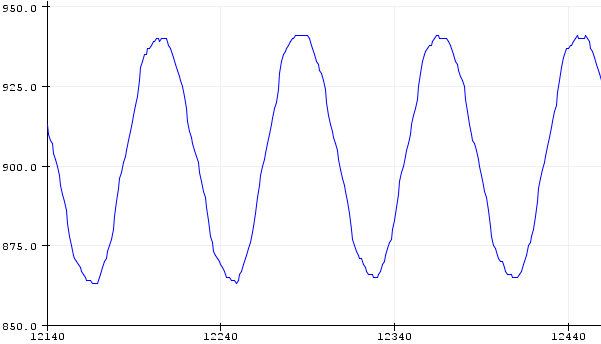
\includegraphics[width=8cm]{ruis.png}
%DIFDELCMD < %%%
%DIFDELCMD < \caption{%
{%DIFAUXCMD
\DIFdelFL{De gedetecteerde ruis, gemeten spanning in functie van de tijd}}
%DIFAUXCMD
%DIFDELCMD < \label{fig:ruis}
%DIFDELCMD < %%%
\DIFdelendFL \DIFaddbeginFL [\DIFaddFL{H}]
  \begin{subfigure}[b]{4.2 cm}
    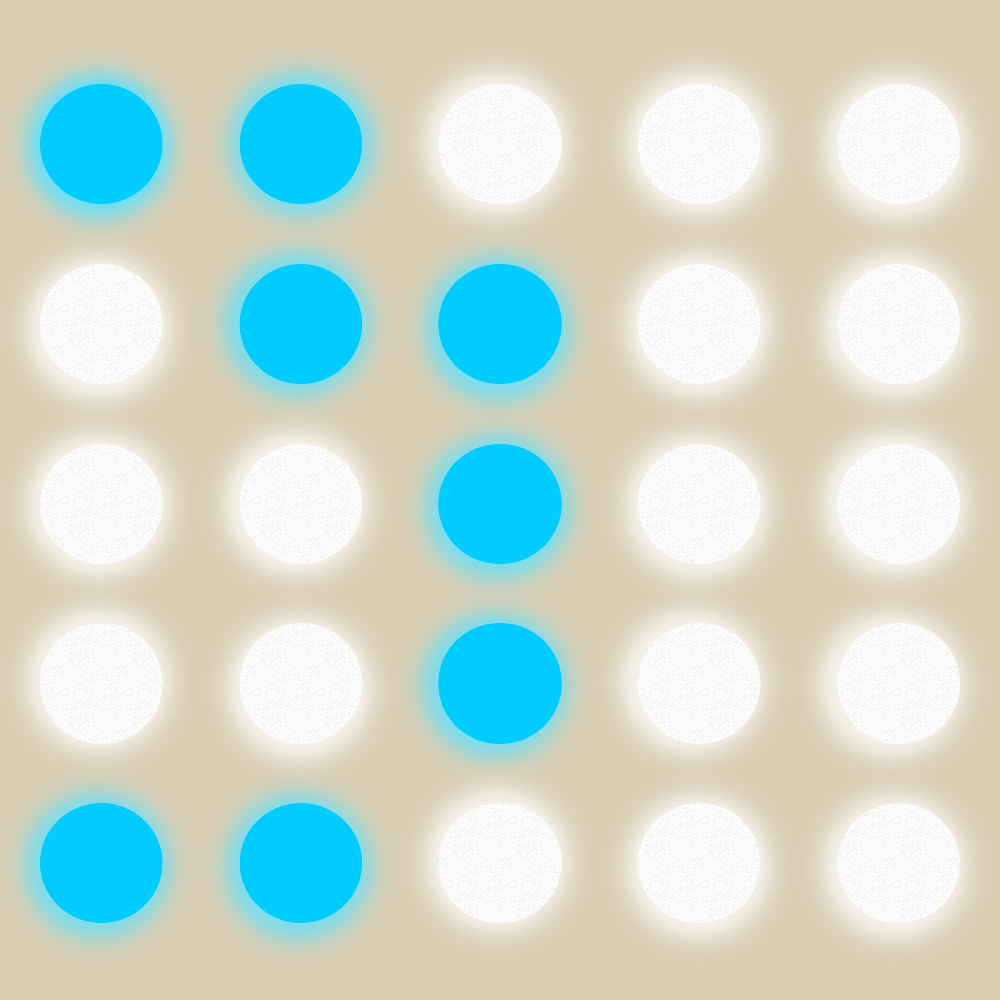
\includegraphics[width=4.2 cm]{Verfborstel.png}
    \caption{\DIFaddFL{Na\"ive implementatie van de verfborstel}}
    \label{verfNaif}
  \end{subfigure}
%DIF > 
    \begin{subfigure}[b]{0.3 cm}
    \end{subfigure}
    %DIF > 
  \begin{subfigure}[b]{4.2 cm}
    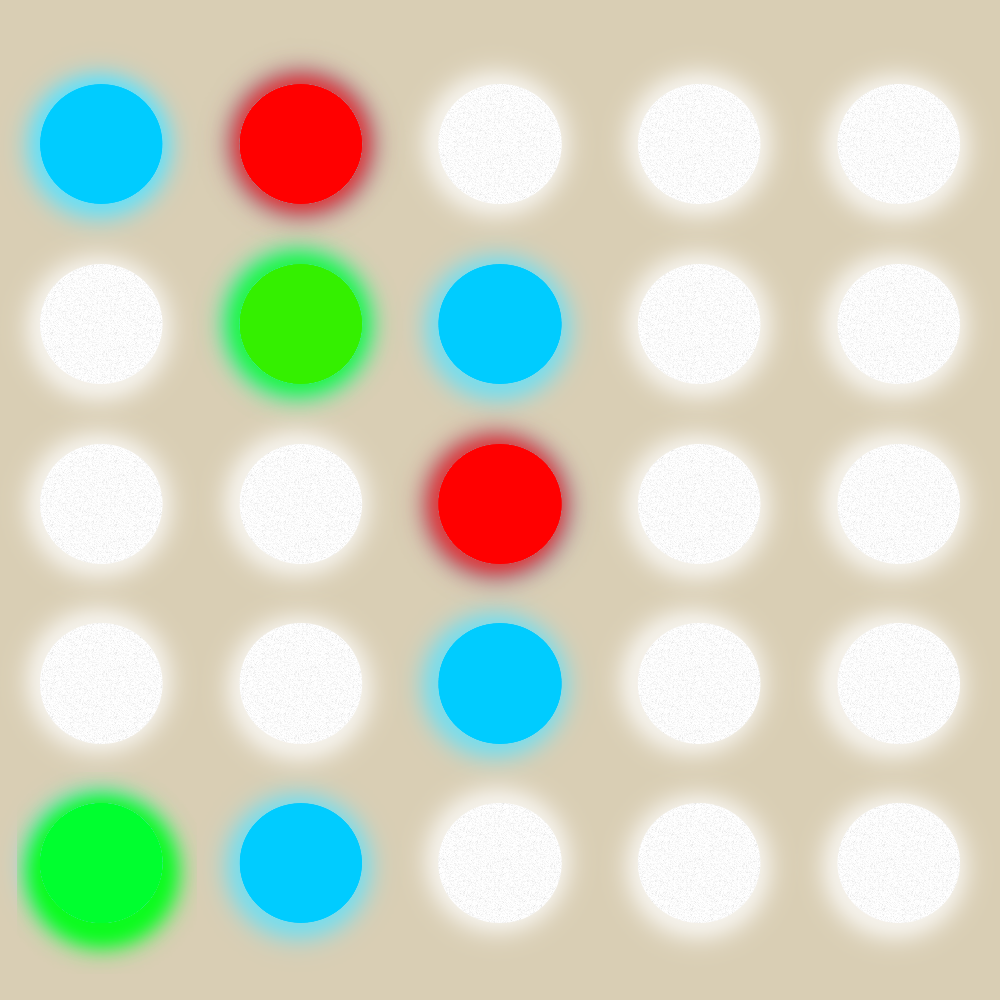
\includegraphics[width=4.2 cm]{VerfborstelKleur.png}
    \caption{\DIFaddFL{Bitstring implementatie van de verfborstel}}
    \label{verfBit}
  \end{subfigure}
\DIFaddendFL \end{figure}

\DIFdelbegin \DIFdel{We merkten op dat deze threshold niet hetzelfde bleef voor eenzelfde hoeveelheid omgevingslicht. Bij het visualiseren van de spanning was te zien dat de gedecteerde ruis sinusoïdaal verloopt (zie figuur \ref{fig:ruis}).
 Dit valt te verklaren door de RC-kringen in de gebruikte zigduino's. Om de gemeten waarde van het omgevingslicht nauwkeuriger te maken besloten we om deze gelijk te stellen aan het gemiddelde van een tiental metingen met telkens 50ms (ongeveer de helft van een periode) tussen om het sinusoïdale verloop op te vangen. Hierbij tellen we opnieuw een waarde op, vergelijkbaar met de amplitude van de sinus golf, en bekomen zo onze threshold.
Dit proces wordt weer meerdere keren herhaald doorheen de uitvoering van het programma. }\DIFdelend \DIFaddbegin \subsubsection{\DIFadd{Programma selecteren}}
\DIFaddend 

\DIFaddbegin \DIFadd{Het is mogelijk om de knoppen een functie te geven buiten de applicatie, bijvoorbeeld om een andere applicatie te selecteren. Zo kan 1 knop gebruikt worden om de SmartLEDs in een “selectie” toestand te brengen. Vanuit deze toestand wachten de display-LEDs op een input om over te schakelen naar het volgende programma. Indien de lichtpen voorzien is van een groter bereik (door meerdere infrarood-LEDs te monteren), zou het mogelijk moeten zijn om de display-LEDs gelijktijdig met een ander programma te laten starten. De synchronisatie zal hier waarschijnlijk niet perfect zijn. Dit is iets waar bij het schrijven van toepassingen rekening moet worden gehouden.
}

\DIFaddend \section{Conclusie}
\DIFdelbegin \DIFdel{We concluderen dat }\DIFdelend \DIFaddbegin 

\DIFadd{We bekijken voor elk van de drie criteria of de SmartLEDs hier geschikt voor zijn en evalueren de andere gevolgen van een SmartLED-display.
 }

\subsection{\DIFadd{Evaluatiecriteria}}
\subsubsection{\DIFadd{Flexibiliteit}}

\DIFadd{Er is geen zijwaartse communicatie tussen de SmartLEDs. Dit zorgt ervoor dat het niet nodig is dat de SmartLEDs op een vaste positie relatief ten opzichte van elkaar staan. Ook verloopt de communicatie onafhankelijk van omgevingsfactoren zoals licht. Het is dus mogelijk om de SmartLED te verplaatsen terwijl het programma loopt. Hieruit besluiten we dat een display opgebouwd uit SmartLEDs voldoet aan onze flexibiliteitscriteria.
}

\subsubsection{\DIFadd{Interactie}}

\DIFadd{De interactie met het display gebeurt aan de hand van een lichtpen voorzien van knoppen. We zijn in staat om verschillende signalen naar het display te sturen en hier visuele feedback vanuit het display op te geven. Door de knoppen te voorzien van bijvoorbeeld gekleurde stickers is de communicatie heel intuïtief; er is weinig of geen uitleg nodig voor een gebruiker om met het display te communiceren. Hieruit besluiten we dat het display voldoet aan onze interactie criteria.
}

\subsubsection{\DIFadd{Modulariteit}}

\DIFadd{De SmartLEDs kunnen een gesimuleerd geheel vormen zonder dat het uitmaakt welke LEDs deel uitmaken van het display. Hierdoor is het mogelijk om SmartLEDs weg te halen of toe te voegen, mits deze dezelfde applicatie uitvoeren. De SmartLEDs zijn onafhankelijk van elkaar. Indien er een SmartLED defect is zal dit zich beperken tot de individuele LED en niet verspreiden over het display. We besluiten dan het SmartLED-display voldoet aan onze modulariteitscriteria.
}

\subsection{\DIFadd{Beperkingen}}
\DIFadd{De manier waarop we het display samenstellen legt enkele beperkingen op wat betreft de mogelijke toepassingen. Het is niet mogelijk om een signaal door te geven in het display; alle SmartLEDs zijn afhankelijk van eigen initiatief of input van de gebruiker. Dit laat niet toe om het SmartLED-display te gebruiker zoals een conventioneel display. 
}

\DIFadd{Daarnaast is ook de resolutie van het display beperkt. De grote van de SmartLEDs laat niet toe om de resolutie van een conventioneel display te benaderen. Wanneer uitgerust met een pingpongbal-diffuser hebben de LEDs een doorsnede van 3.7cm. Hierdoor zijn ze niet geschikt voor gedetailleerde weergaves maar eerder voor globale vormen op grotere afstand.
}

\begin{figure}[H]
\centering
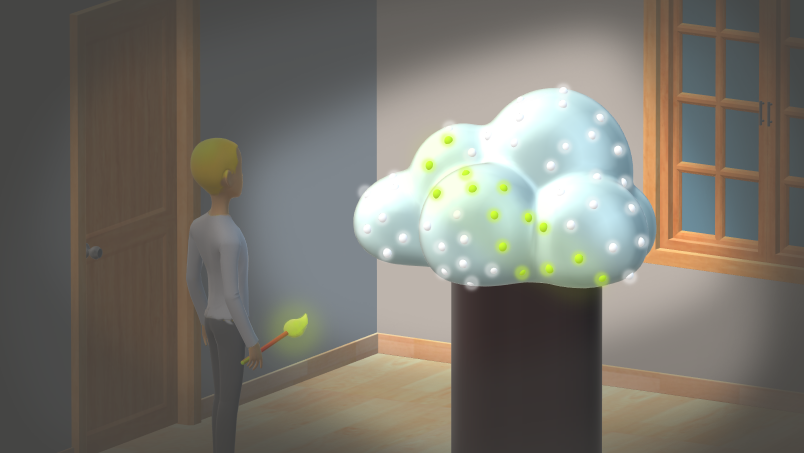
\includegraphics[width=9cm]{MogelijkDisplay.png}
\caption{\DIFaddFL{Artistieke interpretatie van een mogelijk SmartLED-display}}
\label{fig:display}
\end{figure}


\subsection{\DIFadd{Besluit}}

\DIFadd{Door de beperkingen op vlak van zijdelingse communicatie en resolutie zijn de }\DIFaddend SmartLED-displays geen alternatief \DIFdelbegin \DIFdel{zijn voor }\DIFdelend \DIFaddbegin \DIFadd{voor de }\DIFaddend conventionele LED-displays\DIFdelbegin \DIFdel{maar dat ze toch over bepaalde eigenschappen beschikken die ze niet alleen bruikbaar maar ook bijzonder maken }\DIFdelend . 
\DIFdelbegin \DIFdel{Ze kunnen interactief gebruikt worden als simpele, vlakke displays zonder onderlinge communicatie maar ook zonder eventuele verbindingsproblemen. Daarnaast kunnen ze in andere vormen wel signalen doorgeven en dus meer als 1 geheel functioneren}\DIFdelend \DIFaddbegin 

\DIFadd{De eigenschappen op vlak van flexibiliteit, interactie en modulariteit bieden wel mogelijkheden om andere vormen van displays te maken die met conventionele displays technisch moeilijker of duurder te maken zijn. De SmartLED-displays laten toe om het display volledig te vormen rond de oppervlakte waar het op geplaatst wordt. Ook is het mogelijk om tijdens de applicatie de vorm aan te passen en interactie te hebben met het display. Dit laat toe om andere, creatievere displays te maken. Daarom zien wij een toepassingsmogelijkheid van de SmartLED-displays in marketing en entertainment, waar het belangrijk is om uniek en vernieuwend te zijn}\DIFaddend .


\section{Verder werk}
Als vervolg op dit project zou een display opgebouwd uit echte SmartLEDs \DIFaddbegin \DIFadd{(in plaats van de door ons gebruikte Zigduino's) }\DIFaddend gemaakt kunnen worden. Het zou ook interessant zijn \DIFdelbegin \DIFdel{mocht er een oplossing gevonden worden voor het probleem met de invalshoek van de LEDs zodat zijdelings gecommuniceerd kan worden}\DIFdelend \DIFaddbegin \DIFadd{om de mogelijkheden voor zijwaartse communicatie tussen de displayLEDs verder te onderzoeken. Ook zijn er andere applicaties mogelijk waarbij de flexibiliteit van het display verder benut wordt}\DIFaddend .

\DIFdelbegin %DIFDELCMD < \bibliographystyle{named}
%DIFDELCMD < %%%
\DIFdelend \bibliography{bronnen}
\DIFaddbegin \bibliographystyle{named}
\DIFaddend 

\end{document}

